\documentclass{article}
\usepackage{graphicx}
\usepackage{hyperref}

\begin{document}

\title{The HypeDyn Hypertext Fiction Editor\\Tutorial 3: Node Rules and Facts}
% \author{Alex Mitchell}
\date{}

\onecolumn
\maketitle

\tableofcontents


\section{Introduction}
In this tutorial, we will introduce some new features to HypeDyn:

\begin{itemize}
  \item ``node rules'', which allow conditions to be attached to
  \textit{anywhere nodes} as well as links, and allow you to update facts when a
  node is visited; and
  \item ``facts'', which represent information which can be set and checked
  while a story is being read. Facts can be used in conditions, and can also be
  used as alternative text.
\end{itemize}

% We will also be working with a modified version of HypeDyn, which only allows
% \textit{one} non-anywhere node. This is to allow you to focus on the idea of
% hypertext where you do \textit{not} specify links explicitly - instead, you set
% conditions as to when anywhere nodes can be seen using node rules and facts.

% - t/f facts are actually a convenience, could do the same with node/link
% conditions - except, can retract facts selectively, and can simplify if several
% nodes have same outcome
% - text facts also are simply a convenience to reduce using may diff alt texts
% - attempt to encourage procedural thinking
% - node rules let you set facts
% - also let you use anywhere nodes conditionally - sculptural approach
% [add count? add time? add numbers/math?]

In this tutorial, we will be creating a new version of the ``Little Red
Riding Hood'' story, which does not build on the versions created in tutorials
1 and 2. This time, we will be using \textit{anywhere} nodes for all of the
content, and will be making use of the automatic generation of links to these
nodes, plus a combination of \textit{facts} and \textit{node rules} to control
when the reader can see these nodes.

\begin{figure}[h]
  \centering
  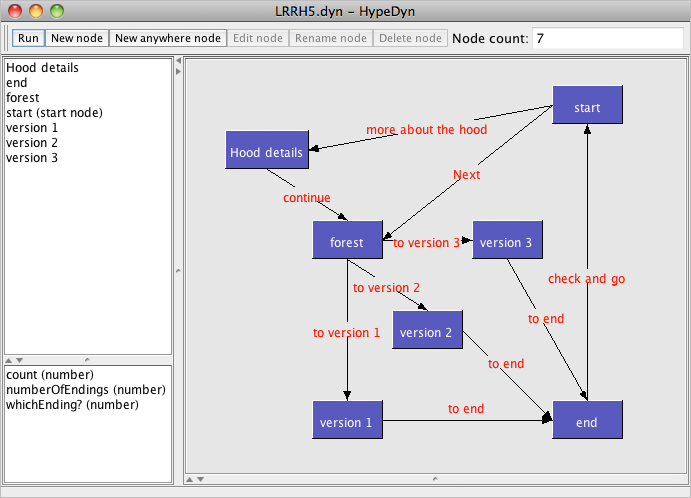
\includegraphics[width=10cm]{images/hypedyn-tutorial-3-figure-1}
  \caption{\textit{The completed ``Little Red Riding Hood'' story.}}
\end{figure} 

The nodes and facts in the final story are shown in Figure 1.

\textit{Note:  HypeDyn is a work-in-progress, so there are some features that are still
not completed, and there may be bugs. If you encounter any errors, please
report them as bugs on our Launchpad site: \url{https://launchpad.net/hypedyn}.}

\section{Getting started}

Make sure that you are working with HypeDyn 2.1s, the customized version of
HypeDyn for NM3222 project 2.

First, open HypeDyn by double-clicking on the file \textbf{HypeDyn.exe} (in
Windows) or \textbf{HypeDyn.app} (in MacOS). Notice that there are some subtle
differences from the version of HypeDyn you used in tutorials 1 and 2 (see
Figure 2). The node list (A) and graph view (D and E) are the same. However,
notice that initially the normal node graph view is much smaller than the
anywhere node graph view. This reflects the fact that you will be writing your
story entirely with anywhere nodes.

Next, notice that there is a new list view below the node list (B) - this is
the \textit{fact list}. There is also a new menu (C) - this is the \textit{fact
menu}. We will come back to these later in the tutorial.

\begin{figure}[h]
  \centering
  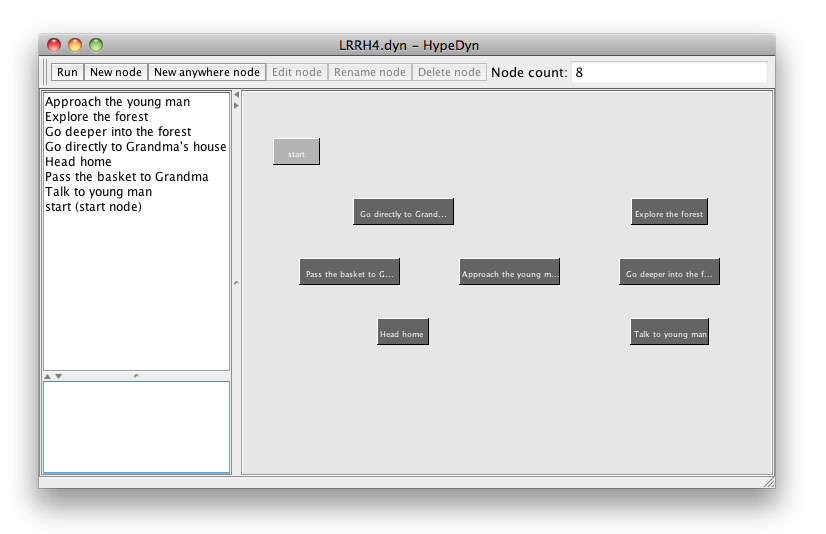
\includegraphics[width=10cm]{images/hypedyn-tutorial-3-figure-2}
  \caption{\textit{The main HypeDyn window.}}
\end{figure} 

Notice that when you open HypeDyn, the new file automatically has one node -
a normal node, which is automatically named ``Start'' and set to be the start
node. Also notice that the \textit{New Node} button is gone. The \textit{New Node} menu
item in the \textit{Nodes} menu is also gone. If you select the ``Start''
node, you'll see that the \textit{Delete node} button is disabled, and the
\textit{Delete node} menu item is also disabled. In this version of HypeDyn, you
cannot create normal nodes, and you cannot delete the one node that was created
for you. All of your story content must be written in \textit{Anywhere} nodes.

\section{Writing ``sculptural'' hypertext}

Writing a story in this version of HypeDyn requires a slightly different way of
thinking about hypertext. Each node, as in regular hypertext, represents a
fragment of the story. Since the nodes you'll be using are \textit{anywhere
nodes}, initially all the nodes will be accessible from every other node -
essentially there are implicit links between every node.

Once your nodes are created, you need to start thinking about restricting the
reader's possible paths through the nodes, otherwise your story will have no
structure, and the reader is likely to become overwhelmed and lost. You will do
this by using \textit{node rules} to determine when an anywhere node's link can
be seen. As you start restricting access, you are essentially removing some of
the implicit links.

This approach is often referred to as ``sculptural'' hypertext
\cite{Bernstein:2001aa,Bernstein:2002aa}, since the process of placing
conditions on the nodes is similar to carving out a sculpture from a block of
stone - what is left behind once unwanted links are carved away is the story

We'll see how this works as we go through and create our version of Little
Red Riding Hood. 

\section{Creating the nodes}
We'll start by creating a collection of nodes which represent the fragments in
the story.

First, edit the ``start'' node, and put in the following content:

\begin{quotation}
One day, Little Red Riding Hood is walking through the forest, on the way to
deliver a basket of food and flowers to her grandmother. 
\end{quotation}

Now create the following set of anywhere nodes:

\begin{enumerate}
  \item \textit{Name}: Explore the forest\\
  \textit{Content}: 
  \begin{quotation}
  Tempted by a grove of flowers, Red strays off the path into the forest. There
  are a number of different types of flowers growing in the grassy clearing.
  \end{quotation}
  \item \textit{Name}: Go deeper into the forest\\
  \textit{Content}: 
  \begin{quotation}
  A handsome young man is leaning against the trunk of a tree. He gestures to
  Red to come over.
  \end{quotation}
  \item \textit{Name}: Talk to young man\\
  \textit{Content}: 
  \begin{quotation}
  Red goes over and talks to the wolf. He asks her where she's going, and she
  says she's off to deliver a basket of food and flowers to her sick grandma. 
  \end{quotation}
  \item \textit{Name}: Go directly to Grandma's house\\
  \textit{Content}: 
  \begin{quotation}
  Red walks along the path, sticking carefully to the center to avoid the dark, menacing trees. Eventually, she reaches Grandma's house.

  When Red enters Grandma's house, she is surprised to see the young man
  sitting on the sofa.
  
  Grandma smiles when she sees Red.
  \end{quotation}
  \item \textit{Name}: Pass the basket to Grandma\\
  \textit{Content}: 
  \begin{quotation}
  Red passes the basket of food and flowers to Grandma.
  \end{quotation}
  \item \textit{Name}: Approach the young man\\
  \textit{Content}: 
  \begin{quotation}
  Unfortunately, the young man was a wolf. Neither Red nor Grandma were ever
  seen again.
  \end{quotation}
  \item \textit{Name}: Head home\\
  \textit{Content}: 
  \begin{quotation}
  Red heads back home.
  \end{quotation}
\end{enumerate}

After creating these nodes, you should have something like what can be seen in
Figure 3. Note that, as there are no links, the arrangement of the nodes in the
graph view is entirely up to you.

\begin{figure}[h]
  \centering
  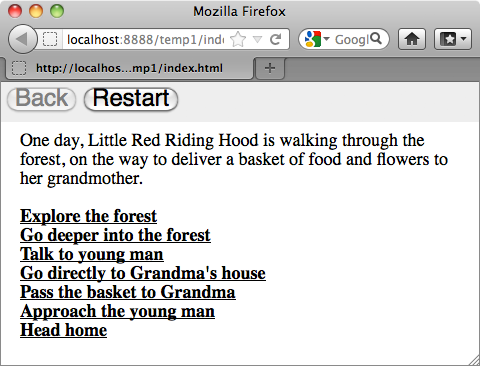
\includegraphics[width=10cm]{images/hypedyn-tutorial-3-figure-3}
  \caption{\textit{The initial set of nodes.}}
\end{figure} 

If you now try running the story, you'll see that all the nodes are available
from all other nodes (see Figure 4). If you click on the links, at each node
all the other nodes are available. We will now start to carve out the shape of
our story using \textit{node rules}.

\begin{figure}[h]
  \centering
  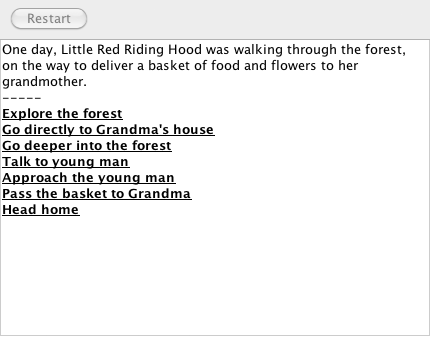
\includegraphics[width=8cm]{images/hypedyn-tutorial-3-figure-4}
  \caption{\textit{Links from every node to every other node.}}
\end{figure} 

\section{Controlling access to nodes using \textit{node rules}}

We will now explore the use of \textit{node rules}. Double-click on the node
``Talk to young man'' in the graph view to open the node editor window. Now go
to the \textit{Edit} menu, and choose the \textit{Edit node rule} menu item.
You will see the \textit{Node rule editor} window (see Figure 5).

\begin{figure}[h]
  \centering
  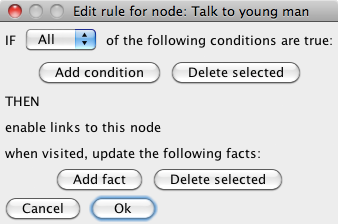
\includegraphics[width=8cm]{images/hypedyn-tutorial-3-figure-5}
  \caption{\textit{The edit node rule window.}}
\end{figure} 

Notice that this window looks similar to the \textit{edit link} window that you
would have seen in tutorials 1 and 2. In fact, both the edit link window and
the edit node rule windows are rule editors. Rules in HypeDyn consist of three
parts: a set of \textit{conditions}, a set of \textit{then} actions which are
carried out if the conditions are true, and a set of \textit{else} actions,
which are carried out if the conditions are \textit{not} true.

In a node rule, the conditions are the same as for a link. The actions,
however, are different. Notice that under the \textit{then} section of the node
rule editor, there are two actions: ``enable links to this node'' and ``when
visited, update the following facts''. We will look at the first of these
actions now, and come back to the second later in the tutorial.

What we want to do at this point is control access to our anywhere nodes. We
can do this by setting conditions in the node rule. If these conditions are
true, then HypeDyn will enable the automatic anywhere links to this node.
Otherwise, the node will not be accessible.

So, what we need to do is think carefully about \textit{when} each of our nodes
should be accessible. One way to think about this is to consider the conditions
on the node to be \textit{preconditions} which must be satisfied for this event
(node) to take place. These preconditions can be expressed in terms of which
other nodes the reader has already seen. For example, for the ``Talk to young
man'' node, we might want this only to be available to the reader if Red has
gone deeper into the forest, ie. the reader has seen the ``Go deeper into the
forest'' node. Lets add this as a condition.

\begin{enumerate}
  \item Click on ``Add condition''.
  \item As in a link, a new condition will appear. If you pull down the
  \textit{Node} pulldown menu, you'll see three options: \textit{Node},
  \textit{Link}, and \textit{Fact}. The first two you've seen before. We'll
  return to the third later.
  \item Choose \textit{Node}, and then choose \textit{Go deeper into the
  forest} and \textit{Visited}.
\end{enumerate}

If you try running the story now, you'll see that although all the other nodes
are still accessible, the node ``Talk to young man'' isn't available until
you've visited ``Go deeper into the forest''.

There is a problem, though - after Red has talked to the young man, and the
reader clicks on any of the other links, the ``Talk to young man'' link
reappears. This can lead to the reader repeatedly looping through the same
node. Although this may sometimes be desirable, particularly if you are using
alternative text to procedurally change the contents of the node, in our story
we don't want this. To prevent this, we can add one more condition to our node:
that the ``Talk to young man'' node itself has \textit{not} been visited.

\begin{enumerate}
  \item Edit the node rule for ``Talk to young man''.
  \item Add another condition, as follows: ``Node Talk to young man Not
  Visited''.
\end{enumerate}

\begin{figure}[h]
  \centering
  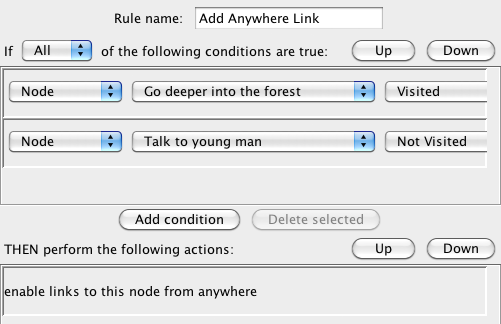
\includegraphics[width=10cm]{images/hypedyn-tutorial-3-figure-6}
  \caption{\textit{The node rule for ``Talk to young man''.}}
\end{figure} 

Your node rule should be similar to what is shown in Figure 6. 

Now if you run the story, the ``Talk to young man'' node is \textit{only}
available after you visit ``Go deeper into the forest'' and haven't yet
visited ``Talk to young man''.

This handles most of the conditions. However, what if the reader had decided
to, for example, click on ``Head home'' or ``Go directly to Grandma's house''?
Would it make sense for Red to still be able to talk to the young man at this
point? Probably not, so we need to add two more conditions.

\begin{enumerate}
  \item Edit the node rule for ``Talk to young man''.
  \item Add another condition, as follows: ``Node Head home Not
  Visited''.
  \item Finally, add the condition ``Go directly to Grandma's house Not
  Visited''.
\end{enumerate}

Your final node rule should be similar to what is shown in Figure 7.

\begin{figure}[h]
  \centering
  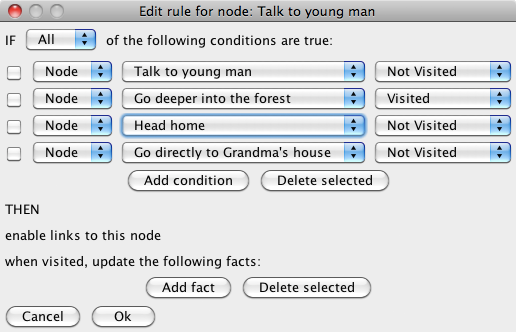
\includegraphics[width=10cm]{images/hypedyn-tutorial-3-figure-7}
  \caption{\textit{The final node rule for ``Talk to young man''.}}
\end{figure} 

\section{Adding the rest of the node rules}

We can now go through and consider each of the other nodes, and add appropriate
conditions. A good way to do this is to work back from the most constrained
nodes to the least constrained nodes. So, working back from ``Talk to young
man'', we can now consider ``Go deeper into the forest''. Logically, this node
should only be available if the reader has chosen to visit ``Explore the
forest'', and should only be seen once. It should also not be available if the
reader has chosen ``Head home'' or ``Go directly to Grandma's house''. To get
this to work, we can follow a similar approach to what we did above.

\begin{enumerate}
  \item Edit the node rule for ``Go deeper into the forest.
  \item Add a condition as follows: ``Node Explore the forest Visited''.
  \item Add another condition as follows: ``Node Go deeper into the forest Not
  Visited''.
  \item Add another condition as follows: ``Node Head home Not
  Visited''.
  \item Finally, add the condition ``Go directly to Grandma's house Not
  Visited''.
\end{enumerate}

The next node we'll consider is ``Explore the forest''. This node is much less
restricted, as we want this to be available to the reader immediately, but only
if it has not yet been visited. As with ``Go deeper into the forest, it should
also not be available if the reader has chosen ``Head home'' or ``Go directly
to Grandma's house''.

\begin{enumerate}
  \item Edit the node rule for ``Explore the forest''.
  \item Add a condition as follows: ``Node Explore the forest Not Visited''.
  \item Add another condition as follows: ``Node Head home Not
  Visited''.
  \item Finally, add the condition ``Go directly to Grandma's house Not
  Visited''.
\end{enumerate}

We have now set out a path for the reader from the start through to talking to
the young man. Next, lets turn our attention to the path to Grandma's house.
The node ``Go directly to Grandma's house'' should always be available
\textit{unless} the reader has already seen it, or has decided to view ``Head
home''.

\begin{enumerate}
  \item Edit the node rule for ``Go directly to Grandma's house''.
  \item Add another condition as follows: ``Node Head home Not
  Visited''.
  \item Finally, add the condition ``Go directly to Grandma's house Not
  Visited''.
\end{enumerate}

Notice that there is also some text in this node which probably should have
conditions attached to it. Following what we did in the previous tutorials, set
it up so that the second paragraph only appears if Red talked to the young man,
and the third paragraph only appears if she \textit{didn't} talk to him.

There are three nodes left: ``Pass the basket to Grandma'', ``Approach the
young man'', and ``Head home''. The first two are important, since they depend
on whether or not Red told the young man where she is going. Because of this,
we need to carefully design their conditions.

For ``Pass the basket to Grandma'', we want the node to be available only if
Red has gone to Grandma's, she \textit{didn't} talk to the wolf, she hasn't gone
home, and she hasn't yet passed the basket to Grandma. This translates into the
following conditions:

\begin{enumerate}
  \item Edit the node rule for ``Pass the basket to Grandma''.
  \item Add the condition ``Go directly to Grandma's house
  Visited''.
  \item Add the condition: ``Node Talk to young man Not Visited''.
  \item Add the condition: ``Node Head home Not Visited''.
  \item Add the condition: ``Node Pass the basket to Grandma Not Visited''.
\end{enumerate}

For ``Approach the young man'' we have a similar set of conditions, although
this time we want to specify that Red \textit{did} talk to the young man.

\begin{enumerate}
  \item Edit the node rule for ``Approach the young man''.
  \item Add the condition ``Go directly to Grandma's house
  Visited''.
  \item Add the condition: ``Node Talk to young man Visited''.
  \item Add the condition: ``Node Head home Not Visited''.
  \item Add the condition: ``Node Approach the young man Not Visited''.
\end{enumerate}

Finally, we have to set the conditions for ``Head home''. This is the least
constrained of all the nodes, as it should be available everywhere
\textit{except} if Red and Grandma were eaten by the wolf.

\begin{enumerate}
  \item Edit the node rule for ``Head home''.
  \item Add the condition: ``Node Approach the young man Not Visited''.
\end{enumerate}

Now run the story. You should be able to explore several variations of the
story, and see that the conditions that we specified ensure that our events
only occur if their preconditions are satisfied.

One thing to note is that we could have achieved a very similar effect using
regular nodes, links, and conditions. However, the \textit{process} of
developing a story using this form of hypertext is very different from what we
saw in tutorials 1 and 2. As a result, the type of story that you are likely to
create is also much different.

It would also be possible to reduce the complexity of the conditions that we
created above by making use of \textit{facts} to keep track of important
information in the story, and use this information to control when nodes are
available. We will now look at how to use \textit{facts}.

\section{Using \textit{facts} to keep track of what has happened}

In previous tutorials, we have seen that HypeDyn can keep track of what the
reader has done by referring to which nodes have been visited, and which links
have been followed. This allows for quite complex procedural change. However,
one major limitaton is that you, as the author, are unable to have HypeDyn
\textit{forget} that a node was visited or a link was followed. There are also
times when a condition depends on one of several nodes having been visited,
which can lead to fairly complex conditions.

To handle these limitations, we will now introduce \textit{facts}. In HypeDyn,
a fact is something which is important to the story. There are two types of
facts: \textit{true/false} facts and \textit{text} facts. \textit{True/false}
facts are either \textit{true} or \textit{false}, and can be checked in a
condition in either a link or a node rule, and updated in a node rule.
\textit{Text} facts contain a piece of text, such as a sentence, can be
updated in a node rule, and can be used to replace text in a node in the same
way as \textit{alternative text}.

Suppose we want to let Red pick the flowers in the forest grove, and put them
in the basket for Grandma. We could do this by using conditions and alternative
text. However, we will now show how this can be done with facts, and then
explain how this is actually more flexible than the approaches used in
tutorials 1 and 2.

First, create two new nodes:

\begin{enumerate}
  \item \textit{Name}: Pick the geraniums\\
  \textit{Content}: 
  \begin{quotation}
  Red decides to pick some of the geraniums in the grove and exchange them for
  the flowers in the basket for Grandma.
  \end{quotation}
  \item \textit{Name}: Pick the violets\\
  \textit{Content}: 
  \begin{quotation}
  Red decides to pick some of the violets in the grove and exchange them for
  the flowers in the basket for Grandma.
  \end{quotation}
\end{enumerate}

We will now create two facts to keep track of whether or not Red has picked the
flowers and which flowers she picked, and one fact to keep track of whether or
not Red is in the forest grove (and therefore able to pick flowers).

\begin{enumerate}
  \item In the main HypeDyn window, go to the \textit{Fact} menu, and pick the
  \textit{New} and \textit{True/False} menu items. 
  \item The ``New True/False Fact'' dialogue will appear (see Figure 8). Enter
  the name of the fact as ``Picked flowers'', and click ``ok''.
  \item Now go to the \textit{Fact} menu, and pick the
  \textit{New} and \textit{True/False} menu items again. 
  \item The ``New True/False Fact'' dialogue will appear. Enter
  the name of the fact as ``In the forest grove'', and click ``ok''.
  \item Now go to the \textit{Fact} menu, and pick the
  \textit{New} and \textit{Text} menu items. 
  \item The ``New Text Fact'' dialogue will appear. Enter
  the name of the fact as ``The flowers'', and click ``ok''.
\end{enumerate}

\begin{figure}[h]
  \centering
  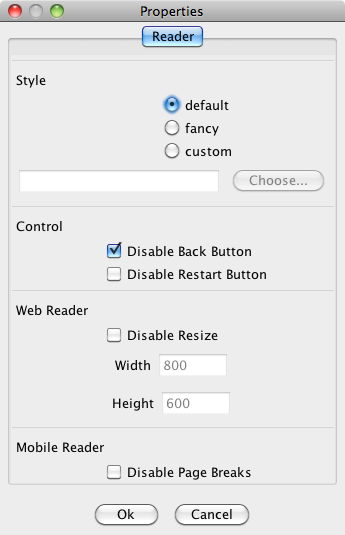
\includegraphics[width=5cm]{images/hypedyn-tutorial-3-figure-8}
  \caption{\textit{Creating a new fact.}}
\end{figure}

We will use the fact ``Picked flowers'' to remember if the reader has had Red
pick the flowers, and ``The flowers'' to remember the type of flowers. We will
use the fact ``In the forest grove'' to make sure that the flowers can only be
picked in the forest grove. This could be done by checking which nodes have and
haven't been visited, but in this case using a fact is much simpler, and allows
for greater flexibility.

Now we need to make sure that the two nodes for picking the flowers are only
available when Red is in the forest grove, and hasn't yet picked the flowers.
We'll do this by using the two \textit{true/false} facts created above.

\begin{enumerate}
  \item Edit the node rule for node ``Pick the violets''.
  \item Add a condition, and select \textit{Fact} as the type. Now choose the
  fact \textit{Picked flowers} and value \textit{False}. This means that the
  condition is true when the fact \textit{Picked flowers} is false, ie. Red
  hasn't picked the flowers. Note that facts are always \textit{false} until
  they have been updated, so when the story is run, both \textit{Picked
  flowers} and \textit{In the forest grove} are false.
  \item Add another condition, and set it to ``Fact In the forest grove True''.
  This means that the condition is true when Red is in the forest grove.
\end{enumerate}

You should have conditions as in Figure 9.

\begin{figure}[h]
  \centering
  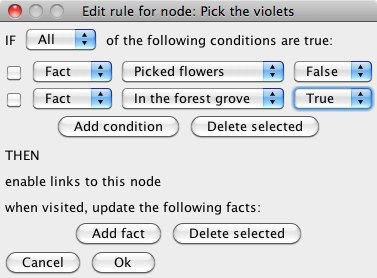
\includegraphics[width=10cm]{images/hypedyn-tutorial-3-figure-9}
  \caption{\textit{Conditions for ``Pick the Violets''.}}
\end{figure}

Now that we have our condition set, we need to update our facts. Facts are
updated when nodes are visited. In the lower half of the \textit{edit node
rule} window, the second action that is carried out when the conditions are
true is to update a list of facts. We'll now set the fact ``Picked flowers'' to
\textit{true} when the reader visits node ``Pick the violets'', and update the
fact ``The Flowers'' to hold the name of the flowers that were picked.

\begin{enumerate}
  \item Edit the node rule for node ``Pick the violets'' again.
  \item Click on \textit{Add fact}, and select \textit{True/False} as the type.
  Now choose the fact \textit{Picked flowers} and set the value
  to \textit{True}. This means that when the node ``Pick the violets'' is
  visited, the fact \textit{Picked flowers} is set to \textit{true},
  ie. Red has picked the flowers.
  \item Click on \textit{Add fact}, and select \textit{Text} as the type.
  Now choose the fact \textit{The flowers}. You should see a text entry field
  appear to the right. Type in the text ``violets''.
\end{enumerate}

The \textit{edit node window} should look something like Figure 10.

\begin{figure}[h]
  \centering
  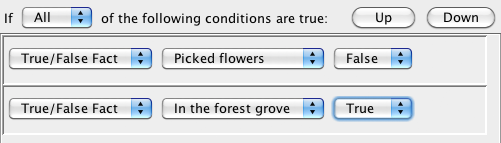
\includegraphics[width=10cm]{images/hypedyn-tutorial-3-figure-10}
  \caption{\textit{Updating facts for ``Pick the Violets''.}}
\end{figure}

Now do exactly the same thing for the node ``Pick the geraniums'', except in
the last step, type in the text ``geraniums'' instead of ``violets''.

At this point we are missing one key step - we don't ever set the fact ``In the
forest grove'' to true. We want to use this to keep track of when the reader
can have Red pick the flowers. To do this, we need to set the fact to
\textit{true} when Red enters the forest, ie. when the reader visits the node
``Explore the forest'', and set it to \textit{false} whenever any of the nodes
which represent leaving the forest grove are visited. These nodes are ``Go
directly to Grandma's house'', ``Head home'', and ``Go deeper into the forest''.

\begin{enumerate}
  \item Edit the node ``Enter the forest''.
  \item Edit its node rule, and add the fact ``In the forest grove'' to the
  list of facts being updated. Set the fact to \textit{true}.
  \item Now do the same for nodes ``Go directly to Grandma's house'', ``Head
  home'', and ``Go deeper into the forest'', but instead of setting the fact to
  \textit{true}, set it to \textit{false}.
\end{enumerate}

We now have the fact set up to track whether Red is in the forest grove or not.
Note that this would be \textit{very} difficult to accomplish using conditions
on whether nodes where visited or not. (Try it!)

The one thing remaining to be done is to update the text where the flowers are
mentioned, so that the specific type of flowers that Red picked are shown.
There are two places where this can be done: ``Pass the basket to Grandma'',
and ``Talk to young man''. We'll to the first, and the second is left as an
exercise.

\begin{enumerate}
  \item Edit the node ``Pass the basket to Grandma''.
  \item Select the text ``flowers'', and create a new link named ``flowers''.
  \item In the link editor, check the checkbox beside ``show alternative text''.
  \item Now change the type of text from ``alternative text'' to ``text from
  Fact'', and choose the fact \textit{The flowers}.
\end{enumerate}

This means that the link text will be replaced by whatever value for the fact
``The flowers'' we have set it to - either ``violets'' or ``geraniums'',
depending on which node the reader visited. We also need to make sure this
replacement is only done if the flowers have been picked:

\begin{enumerate}
  \item In the link editor, add a condition, and select type \textit{Fact}.
  Choose the fact \textit{Picked flowers}, and the value \textit{False}. This
  means that the default text will be shown if the flowers have \textit{not}
  been picked, and the value of the fact \textit{The flowers} will be shown if
  the flowers \textit{have} been picked.
\end{enumerate}

The link for the alternative text should look something like Figure 11.

\begin{figure}[h]
  \centering
  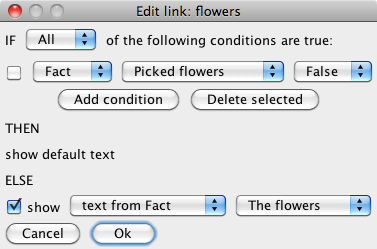
\includegraphics[width=10cm]{images/hypedyn-tutorial-3-figure-11}
  \caption{\textit{Substituting alternative text with a fact.}}
\end{figure}

Try running the story and picking the flowers. Notice that for either of the
flowers that are picked, the correct name is substituted in the node ``Pass the
blanket to Grandma''. Try adding the same alternative text to the node ``Talk
to young man''.

Note that, as with the other examples where we have used facts, we could have
done the same thing with regular node conditions and alternative text. However,
it would have required several links in the ``Pass the basket to Grandma''
node. In addition, we can easily add a third flower, and no changes need to be
made to either of the nodes where the text is substituted. This allows for much
more systematic use of procedural change than the alternative text mechanism
introduced in earlier tutorials.

\section{Next steps}

We have created a simple story using the ``sculptural'' approach to hypertext,
where all nodes implicitly have links between them, and the creation of the
story structure consists of using conditions to gradually restrict which nodes
are and are not available to the reader. We have also used facts to keep track
of what the reader has done, and to procedurally change the text in nodes. The
completed version of this story can be found in the file \textsc{LRRH4.dyn}.

There are several things that you could try to enhance the story. For example,
you could allow the reader to go back from ``Go deeper into the forest'' to pick
the flowers. This can easily be done by making use of the ``In the forest grove''
fact. Try adding a third type of flower to be picked. You might also want to go
back and use facts instead of node conditions to simplify the conditions we
placed on the anywhere nodes in the first part of this tutorial.

\section{Conclusion}

In this tutorial, we have created a simple ``sculptural'' hypertext fiction. By
creating a collection of story fragments, and then specifying a set of
conditions for when these fragments can be seen, we have taken a very different
approach to writing a hypertext story than was seen in the earlier versions of
HypeDyn. In addition, by using \textit{facts} to keep track of what the reader
has done, either as true or false conditions, or as text, we now have a much
more flexible way of changing the behaviour of the system based on the reader's
actions. This provides more much more powerful possibilities in terms of
procedural change and interactivity.

% \section{Final notes}
% 
% As mentioned above, the HypeDyn hypertext editor is still a work-in-progress.
% Please let me know if you encounter any problems. Also, please post your
% questions about using the tool to the IVLE forum.

  \bibliographystyle{apalike}
  \bibliography{../../../../../Research/references/papers/thesis}

\end{document}
